\documentclass{beamer}
\usetheme{tumkdd} %  TUM KDD beamer theme (beamerthemetumkdd.sty)

\usepackage{graphicx}
\usepackage{pgfplots}         % Plots in Latex
\usepackage{amsmath, amssymb} % Math formulas and symbols
\usepackage{tikz}
\usetikzlibrary{arrows}

\title[Passing and propagation]{Message passing and expectation propagation}
%\subtitle{Presentation subtitle}
\date{29 May 2017}
\author{Christoph Dehner}
\institute[TUM]
{Technische Universit\"at M\"unchen\\
Department of Informatics\\
Data Mining and Analytics\\
\textcolor{tum}{\url{kdd.in.tum.de}}\\
}

\begin{document}
\begin{frame}
    \titlepage
    \thispagestyle{empty}
\end{frame}



\begin{frame}{Motivation}
	Graphical models: Markov random fields, Bayesian networks 
	2 examples
	inference algorithms: exact by message passing
	approximate by expectation propagation
\end{frame}

\begin{frame}{Message passing: Idea}
	~\\
	Bayesian network: $p(X) =  p(x_1) p(x_2|x_1) p(x_3|x_1)$\\
	\begin{figure}
	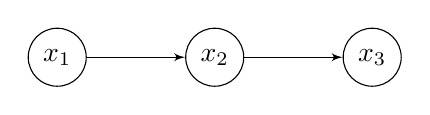
\begin{tikzpicture}
	
	\tikzset{vertex/.style = {shape=circle,draw,minimum size=1.3em}}
	\tikzset{edge/.style = {->,> = latex'}}
	
	\node[vertex] (x1) at  (0,0) {$x_1$};
	\node[vertex] (x2) at  (2,0) {$x_2$};
	\node[vertex] (x3) at  (4,0) {$x_3$};
	
	\draw[edge] (x1) to (x2);
	\draw[edge] (x2) to (x3);
	\end{tikzpicture}
	\end{figure}
	
	Marginalization naive:
	\begin{equation*}
	p(x_2)= \sum_{X \setminus x_2} p(X)
	\end{equation*}
	Marginalization advanced:
	\begin{equation*}
	\begin{split}
	p(x_2) &= \sum_{x_1} \sum_{x_3} p(x_1) p(x_2|x_1) p(x_3|x_2) \\ &= \underbrace{\Big[ \sum_{x_1}  p(x_1) p(x_2|x_1)\Big]}_{\mu_{x_1 \rightarrow x_2}}\cdot \underbrace{\Big[ \sum_{x_3}  p(x_3|x_2)\Big]}_{\mu_{x_3 \rightarrow x_2}}
	\end{split}
	\end{equation*}
\end{frame}

\begin{frame}{Factor graph}
	Bayesian network: $p(X) =  p(x_1) p(x_2|x_1) p(x_3|x_1)$\\
	\begin{figure}
		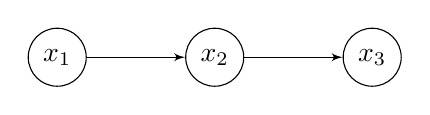
\begin{tikzpicture}
		
		\tikzset{vertex/.style = {shape=circle,draw,minimum size=1.5em}}
		\tikzset{edge/.style = {->,> = latex'}}
		
		\node[vertex] (x1) at  (0,0) {$x_1$};
		\node[vertex] (x2) at  (2,0) {$x_2$};
		\node[vertex] (x3) at  (4,0) {$x_3$};
		
		\draw[edge] (x1) to (x2);
		\draw[edge] (x2) to (x3);
		\end{tikzpicture}
	\end{figure}
	
	Corresponding factor graph:
	\begin{figure}
		\centering
		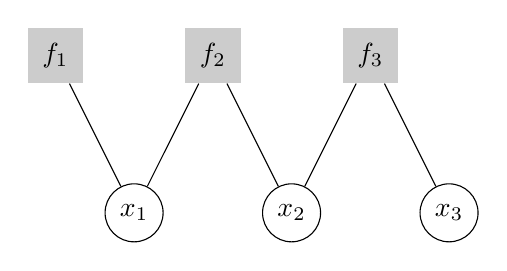
\begin{tikzpicture}
			\tikzset{vertex/.style = {shape=circle,draw,minimum size=1.5em}}
			\tikzset{edge/.style = {-,> = latex'}}
			
			\node[vertex] (x1) at  (0,0) {$x_1$};
			\node[vertex] (x2) at  (2,0) {$x_2$};
			\node[vertex] (x3) at  (4,0) {$x_3$};
			
			\tikzset{vertex/.style = {shape = rectangle,fill = gray!40,minimum size=2em}}
			\node[vertex] (f1) at  (-1,2) {$f_1$};
			\node[vertex] (f2) at  (1,2) {$f_2$};
			\node[vertex] (f3) at  (3,2) {$f_3$};
			
			\draw[edge] (x1) to (f1);
			\draw[edge] (x1) to (f2);
			\draw[edge] (x2) to (f2);
			\draw[edge] (x2) to (f3);
			\draw[edge] (x3) to (f3);
		\end{tikzpicture}
	\end{figure}
\end{frame}

\begin{frame}{Sum-product algorithm}
	General marginalization:
	\begin{equation*}\label{eq:message1}
	\begin{split}
	p(x_i) &= \sum_{X \setminus x_i} \Big[ \prod_{s \in ne(x_i)} F_s(x_i, X_s) \Big] = \prod_{s \in ne(x_i)} \Big[ \underbrace{\sum_{X_s} F_s(x_i, X_s)}_{\mu_{f_s \rightarrow x_i}(x_i)}\Big]% =: \prod_{s \in ne(x_i)} \mu_{f_s \rightarrow x_i}(x_i)
	\end{split}
	\end{equation*}
	Local messages through factor graph:
	\begin{equation*}
	\begin{split}
		\mu_{f_s \rightarrow x_i}(x_i) &= \sum_{\mathbf{x_s} \setminus x_i} f_s(x_i, X_s) \prod_{m \in ne(f_s) \setminus x_i} \mu_{x_m \rightarrow f_s}(x_m)\\
		\mu_{x_m \rightarrow f_s}(x_m) &= \prod_{l \in ne(x_m) \setminus f_s} \mu_{f_l \rightarrow x_m}(x_m)
	\end{split}
	\end{equation*}
	
	Initialization at leaf nodes:
	$\mu_{x \rightarrow f}(x) = 1$, $\mu_{f \rightarrow x}(x) = f(x)$
\end{frame}

\begin{frame}{Max-sum algorithm}
	Maximum aposteriori estimate:
	\begin{equation*}\label{eq:map_problem}
	X^* = \underset{X}{\arg\max}~ p(X) = \underset{X}{\arg\max}~ \ln (p(X))
	\end{equation*}
	Infer $p(X^*)$ by adapting sum-product algorithm:
	\begin{equation*}
	\begin{split}
	\mu_{f_s \rightarrow x_i}(x_i) &= \max_{X_s \setminus x_i} \Big[f_s(x_i, X_s) \sum_{m \in ne(f_s) \setminus x_i} \mu_{x_m \rightarrow f_s}(x_m) \Big]\\
	\mu_{x_m \rightarrow f_s}(x_m) &= \sum_{l \in ne(x_m) \setminus f_s} \mu_{f_l \rightarrow x_m}(x_m)
	\end{split}
	\end{equation*}
	Initialization at leaf nodes:
	$\mu_{x \rightarrow f}(x) = 0$, $\mu_{f \rightarrow x}(x) = \ln f(x)$
\end{frame}

\begin{frame}{Message passing: Discussion}
	\begin{itemize}
		\item Linear complexity in the number of involved variables
		\item Only exact for trees
		\item In general graphs: Loopy belief propagation
		\item (Linearized message passing)
	\end{itemize}
\end{frame}

\begin{frame}{Expectation propagation: Methodology}
	Approximate posterior distribution:
	\begin{equation*}
	p(\theta|\mathbf{D}) = \frac{1}{p(\mathbf{D})} p(\theta, \mathbf{D}) = \frac{1}{p(\mathbf{D})} \prod_i f_i(\theta , \mathbf{D})
	\end{equation*}
	Approximating function from exponential family:
	\begin{equation*}
	q(\theta) = \frac{1}{Z}\prod_i \tilde{f}_i(\theta)
	\end{equation*}
	Minimize KL divergence $KL(p||q)$: Moment matching!
\end{frame}

\begin{frame}{Expectation propagation: Algorithm}
	Approximating function:
	\begin{equation*}
	q(\theta) = \frac{1}{Z}\prod_i \tilde{f}_i(\theta)
	\end{equation*}
	Iteratively refine one factor at a time:
	\begin{equation*}
	\begin{split}
	q^{\backslash j}(\theta) &= \prod_{i\ne j} \tilde{f}_i(\theta)\\
	q^{new}(\theta) & \propto f_j ~ q^{\backslash j}(\theta)\\
	\tilde{f}_j &= \frac{1}{Z_j} \frac{q^{new}(\theta)}{q^{\backslash j}(\theta)}
	\end{split}
	\end{equation*}

\end{frame}

\begin{frame}{Expectation propagation: Discussion}
	\begin{itemize}
		\item Can be applied to general distribution
		\item Expectation propagation is not guaranteed to converge
		\item If EP converges, it often outperforms VI
	\end{itemize}

\end{frame}

\begin{frame}{EP vs. VI}
	Expectation propagation: Minimize $KL(p||q) = \int p \ln \frac{p}{q}$\\
	~\\
	Variational inference: Minimize $KL(q||p)  = \int q \ln \frac{q}{p}$
	\begin{figure}[h]
		\begin{center}
			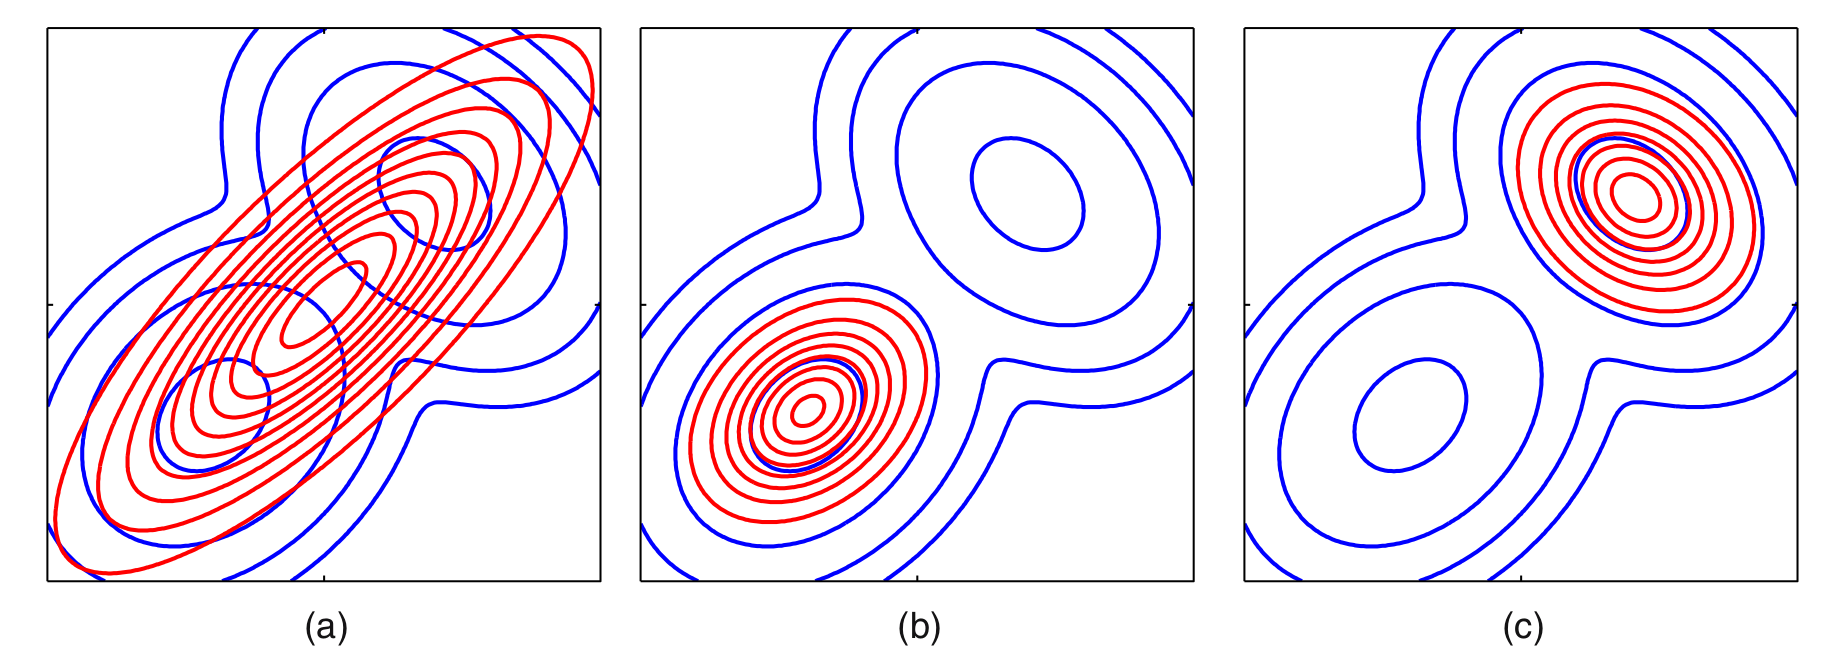
\includegraphics[scale=0.15]{../multimodal_approximation.png}
		\end{center}
	\end{figure}
	\small{Figure taken from Bishop: Pattern Recognition and Machine Learning.}
	
\end{frame}

\begin{frame}{}
	\centering
    Thanks for your attention!\\
    Questions?
\end{frame}


\end{document}
